\documentclass{article}

% NeurIPS-style single-column preprint, self-contained so it compiles with pdflatex.
% To submit, drop the body into the official neurips_2024.tex (\usepackage{neurips_2024}).
\usepackage[letterpaper,margin=1.25in]{geometry}
\usepackage{times}
\usepackage{amsmath,amssymb}
\usepackage{booktabs}
\usepackage{array}
\usepackage{graphicx}
\usepackage{tikz}
\usetikzlibrary{positioning,arrows.meta}
\usepackage{microtype}
\usepackage[colorlinks=true,allcolors=blue]{hyperref}
\usepackage{xcolor}
\usepackage{titlesec}
\titleformat{\section}{\normalfont\large\bfseries}{\thesection}{0.6em}{}
\titleformat{\subsection}{\normalfont\normalsize\bfseries}{\thesubsection}{0.6em}{}
\setlength{\parindent}{0pt}\setlength{\parskip}{0.5em}
\renewcommand{\topfraction}{0.9}\renewcommand{\bottomfraction}{0.8}
\renewcommand{\textfraction}{0.08}\renewcommand{\floatpagefraction}{0.75}
\setcounter{topnumber}{3}\setcounter{bottomnumber}{2}\setcounter{totalnumber}{5}
\newcommand{\KL}{\mathrm{KL}}
% frame thumbnail with a build-safe fallback box if the image hasn't been extracted yet
\newcommand{\frm}[1]{\IfFileExists{figures/#1}{\includegraphics[height=14mm]{figures/#1}}%
  {\fbox{\parbox[c][13mm][c]{17mm}{\centering\scriptsize\ttfamily #1}}}}
\newcommand{\frmrow}[1]{\frm{#1_1.jpg}\hspace{1.2pt}\frm{#1_2.jpg}\hspace{1.2pt}\frm{#1_3.jpg}}
\newcommand{\exrow}[5]{%
  \begin{tikzpicture}[font=\footnotesize,>={Latex[length=1.8mm]}]
    \node[draw=black!30,rounded corners=2.5pt,inner sep=1.6pt,line width=0.5pt] (im) {\frmrow{#1}};
    \node[anchor=west,align=left,text width=52mm,inner sep=0pt] (c)
      at ([xshift=8mm]im.east) {#2\\[2.5pt]\emph{#3}};
    \draw[->,black!45,line width=0.7pt] (im.east) -- (c.west);
    \node[draw=red!60!black,fill=red!8,rounded corners=3pt,inner sep=3pt,anchor=north west]
      (b) at ([yshift=-4pt]c.south west) {\color{red!72!black}\,base: #4 \,$\boldsymbol{\times}$\,};
    \node[draw=green!45!black,fill=green!12,rounded corners=3pt,inner sep=3pt,anchor=west]
      (o) at ([xshift=3mm]b.east) {\color{green!48!black}\,ours: #5 \,$\boldsymbol{\checkmark}$\,};
  \end{tikzpicture}}

\title{\textbf{Preference-Optimization Collapse in Frozen Audio--Visual LLMs\\
and a Two-Anchor Mitigation}}
\author{Anonymous}
\date{}

\begin{document}
\maketitle

\begin{abstract}
Audio--visual LLMs under-use audio: they answer from the image, hallucinating sounds it implies and
ignoring sounds that contradict it. We ask whether a \emph{frozen} model can be re-grounded by training
only a small per-modality transform on its adapter token streams, with a modality-conditional preference
--- on an audio-swapped counterfactual, prefer the answer matching the \emph{heard} event over the
\emph{seen} one. Plain direct preference optimization (DPO) on this signal collapses the model: perception
accuracy falls to near zero and the output becomes a near-constant answer. We trace the collapse to
likelihood displacement and the absence of any constraint on the output distribution, and prevent it with
two anchors --- a floor holding the chosen answer's likelihood at the frozen base, and a KL penalty to the
base on general inputs --- with an ablation showing both are necessary. This diagnosis and fix is our main
result. The downstream grounding effect is real but backbone-dependent: under a paired, leakage-controlled
protocol the audio-hallucination probe improves significantly on both Qwen backbones and on every seed,
yielding a net benchmark gain on Qwen3-Omni, a redistribution toward audio (at audio--video matching's
expense) on Qwen2.5-Omni, and a regression on VideoLLaMA2, whose audio pathway is too weak to exploit. A
per-token probe shows the learned transform reshapes the \emph{vision} stream, so the frozen language
model --- not the audio path --- resolves the conflict. We do not claim state of the art.
\end{abstract}

\section{Introduction}
Audio--visual large language models attach pretrained audio and vision encoders to a language model through
lightweight per-modality adapters, and they inherit a modality imbalance: they answer from the visual
stream, hallucinating sounds the image implies and ignoring sounds that contradict it~\cite{cmm,avhbench}.
We ask whether this can be corrected without touching the model --- freezing every pretrained weight and
training only a small per-modality transform on the adapter token streams.

The training signal is a modality-conditional preference. From a clean clip we build an audio-swapped
counterfactual (the original video with another clip's audio) and prefer the answer consistent with the
\emph{heard} event over the \emph{seen} one. Scored on the same swapped clip, this preference can be
satisfied only by attending to the audio.

Our contributions are three. (i)~Plain preference optimization of this objective collapses a frozen
AV-LLM; we trace the collapse to likelihood displacement and a missing output-distribution constraint.
(ii)~Two anchors --- a chosen-likelihood floor and a KL-to-base penalty --- prevent it, and an ablation
shows both are necessary; this is our main, reproducible result. (iii)~Under a paired, leakage-controlled
protocol the adapter redirects grounding toward audio to a backbone-dependent degree, and a per-token
probe locates the change. We do not claim state of the art.

\section{Architecture}
\label{sec:arch}

\begin{figure}[tb]
\centering
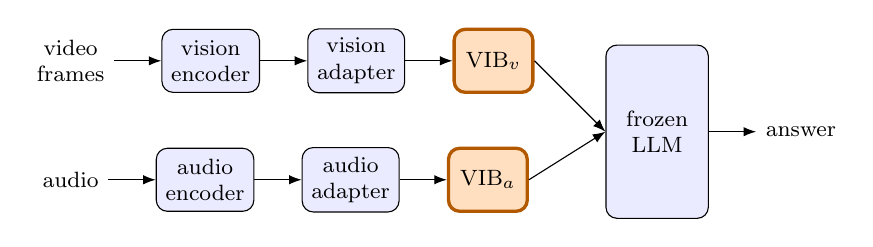
\begin{tikzpicture}[font=\footnotesize,>={Latex[length=1.6mm]},node distance=5mm and 6mm,
  enc/.style={draw,rounded corners,fill=blue!8,minimum width=12mm,minimum height=8mm,align=center},
  vib/.style={draw,very thick,rounded corners,fill=orange!25,draw=orange!70!black,minimum width=10mm,minimum height=8mm,align=center},
  llm/.style={draw,rounded corners,fill=blue!8,minimum width=13mm,minimum height=22mm,align=center},
  io/.style={align=center}]
  \node[io] (vin) {video\\frames};
  \node[enc,right=of vin] (venc) {vision\\encoder};
  \node[enc,right=of venc] (vproj) {vision\\adapter};
  \node[vib,right=of vproj] (vvib) {$\mathrm{VIB}_v$};
  \node[io,below=9mm of vin] (ain) {audio};
  \node[enc,right=of ain] (aenc) {audio\\encoder};
  \node[enc,right=of aenc] (aproj) {audio\\adapter};
  \node[vib,right=of aproj] (avib) {$\mathrm{VIB}_a$};
  \node[llm,right=9mm of vvib,yshift=-9mm] (llm) {frozen\\LLM};
  \node[io,right=of llm] (ans) {answer};
  \draw[->] (vin)--(venc); \draw[->] (venc)--(vproj); \draw[->] (vproj)--(vvib); \draw[->] (vvib.east)--(llm.west);
  \draw[->] (ain)--(aenc); \draw[->] (aenc)--(aproj); \draw[->] (aproj)--(avib); \draw[->] (avib.east)--(llm.west);
  \draw[->] (llm.east)--(ans);
\end{tikzpicture}
\caption{The architecture. Everything blue is frozen; the only trained parameters are the two variational
information bottlenecks (orange) inserted on the per-modality adapter outputs ---
$z=\mu(x)+\sigma(x)\,\epsilon$, $y=x+W_{\text{out}}z$ with $W_{\text{out}}$ zero-initialized (identity at
start). They are trained by an audio-swap preference with two anchors (Section~\ref{sec:method}).}
\label{fig:method}
\end{figure}

The model is frozen. On each per-modality adapter output --- the token sequence $x\in\mathbb{R}^{T\times d}$
feeding the language model --- we attach a variational information bottleneck (VIB) through a forward hook:
\begin{equation}
z=\mu(x)+\sigma(x)\odot\epsilon,\ \epsilon\sim\mathcal N(0,I);\qquad y=x+W_{\text{out}}z,
\end{equation}
with per-token rate $\KL(q(z|x)\,\|\,\mathcal N(0,I))$. Because $W_{\text{out}}$ is zero-initialized the
adapter is the identity at start, and a bypass flag restores the exact frozen base --- which we reuse for
the DPO reference log-probabilities and the KL-to-base target, so no second model is needed. Only the two
VIBs are trained. They attach at the audio-tower projection and vision merger of the Qwen-Omni backbones,
and at the BEATs and SigLIP adapters of VideoLLaMA2.1-7B-AV.

\section{Method: objective and losses}
\label{sec:method}
\textbf{Audio-swap preference and the naive objective.} From each clip we form a multiple-choice question
and an audio-swapped copy (video unchanged, audio from a different-category clip); the chosen letter names
the heard event, the rejected the seen one, both scored on the swapped clip. With $c_p,r_p$ the policy
log-probs of the two letters (bottleneck active) and $c_r,r_r$ the reference (bypassed), the naive
objective regularizes only the latent rate:
\begin{equation}
\mathcal L_0=-\log\sigma\!\big(\beta[(c_p-c_r)-(r_p-r_r)]\big)+\beta_{kl}\,\KL_{\text{VIB}}.
\label{eq:naive}
\end{equation}
Nothing ties the output to the base. As a log-sigmoid of a difference, $\mathcal L_0$ can be reduced by
lowering \emph{both} letter probabilities, and with an always-on adapter and an input-blind objective the
mass drifts to a constant answer.

\textbf{Anchored swap-DPO.} We add two terms:
\begin{align}
\mathcal L=\ &-\log\sigma\!\big(\beta[(c_p-c_r)-(r_p-r_r)]\big)
 +\lambda_{a}\,\big(\!-\log\sigma(\beta(c_p-c_r)-\delta)\big)\nonumber\\
 &+\lambda_{kl}\,\KL\!\big(p_{\text{base}}(\cdot|x)\,\|\,p_\theta(\cdot|x)\big)+\beta_{kl}\,\KL_{\text{VIB}}.
\label{eq:anchored}
\end{align}
The chosen anchor ($\delta{=}0$)~\cite{mdpo,dpop} keeps the chosen log-prob from falling below the frozen
base. The KL-to-base term penalizes drift from the base's answer distribution on general (non-swap) inputs
--- matched multiple-choice, audio- and visual-presence, and open-ended prompts (the ``broad'' set) --- and
is free because the base is the bypassed bottleneck.

\textbf{Monitoring, selection, and numerics.} Throughout training we log the absolute chosen/rejected
log-probs (not only their margin), both KL terms, and the yes-rate on a balanced probe --- a
constant-answer detector --- and select checkpoints on held-out benchmarks by best hallucination accuracy
subject to capability guards (Section~\ref{sec:setup}). Numerically, the VIB runs in float32 (bfloat16
underflows its squared-mean rate term) with normalized input and gradients clipped to norm $1.0$;
VideoLLaMA2's float16 forward overflows attention, so we train it in bfloat16. These guards leave the Qwen
backbones unchanged.

\section{Experimental setup}
\label{sec:setup}
\textbf{Backbones and training.} Qwen3-Omni (primary), Qwen2.5-Omni, and VideoLLaMA2.1-7B-AV, all frozen
with only the two VIBs trained on $300$ audio-swapped AVE preference pairs for two epochs
($\lambda_a{=}1$, $\lambda_{kl}{=}2$, $\beta_{kl}{=}0.01$). \textbf{Selection (leakage control).} We select
checkpoints and hyperparameters on a $300$-example development split of each benchmark and report \emph{all}
final numbers on the disjoint held-out remainder (AVHBench contributing $n{=}5002$). The rule is the best
validation hallucination accuracy subject to capability guards
$\text{PA}\ge\text{PA}_{\text{base}}-0.05$, $\text{HR}\ge\text{HR}_{\text{base}}-0.05$. The ablation
(Table~\ref{tab:abl}) uses the $300$-example diagnosis split; the global comparison
(Table~\ref{tab:main}) uses the held-out remainder. \textbf{Answer parsing.} A negation-aware parser maps
free text to yes/no (e.g.\ ``I did not see a tree''$\,\to\,$``no''); a negation-blind parser had floored
VideoLLaMA2's resistance, as it answers in full sentences while the Qwen backbones lead with
``yes''/``no''. We re-derived every metric from saved outputs, which left all Qwen numbers unchanged.
\textbf{Statistics.} Base and adapted see identical items, so every comparison is a \emph{paired} McNemar
test on the discordant pairs, with bootstrap $95\%$ CIs and seed variance reported in text.

\section{Benchmarks}
\label{sec:bench}
\textbf{AVHBench}~\cite{avhbench} measures cross-modal hallucination through three yes/no tasks ---
audio-driven \emph{video} hallucination ($A\!\to\!V$: is a queried object visible?), video-driven
\emph{audio} hallucination ($V\!\to\!A$: is a queried sound audible?), and audio--video matching; $V\!\to\!A$
is our direct audio-grounding probe. \textbf{CMM}~\cite{cmm} separates perception accuracy (PA; affirming
present content) from hallucination resistance (HR; denying absent content), with over-reliance subsets
(e.g.\ \texttt{overrely\_visual\_ignore\_audio}) that test whether a model ignores one modality for
another. \textbf{DAVE}~\cite{dave} is an audio--visual multiple-choice diagnostic. As reference points we
also evaluate two frozen frontier models: Gemini (native audio--visual) and GPT-4o (vision-only, hence
blind to non-speech sound).

\section{Results and comparisons}
\label{sec:results}
Table~\ref{tab:main} reports full-set accuracy for every model; significance below is the held-out paired
McNemar test. The adapter's robust, seed-invariant effect is the audio probe $V\!\to\!A$: it rises on both
Qwen backbones (Qwen3-Omni $0.787\to0.815$, Qwen2.5-Omni $0.690\to0.780$), significantly on \emph{every}
seed ($p<0.05$), and the CMM over-reliance subset that tests ignoring audio improves on all three
backbones --- the model stops ignoring what it hears.

The benchmarks then diverge by backbone. On Qwen3-Omni the audio gain comes with a matching gain
($0.609\to0.693$), so overall AVHBench rises ($0.714\to0.757$, significant held-out, pooled $p<10^{-4}$).
On Qwen2.5-Omni the audio gain is larger but trades against matching ($0.755\to0.682$), so overall AVHBench
barely moves ($0.737\to0.754$, neutral when pooled) while audio hallucination-resistance climbs
(HR $0.512\to0.559$, $p<10^{-4}$): the adapter \emph{redistributes} grounding toward audio rather than
lifting every axis. On VideoLLaMA2 it instead regresses --- AVHBench $0.715\to0.669$, the audio probe
$0.766\to0.721$ --- consistent with a weak, separately-aligned audio pathway~\cite{avllm_seehear,fastav}
that offers little audio signal to exploit. Among the frozen frontier baselines, native-audio Gemini
reaches $V\!\to\!A{=}0.747$, which adapted Qwen3-Omni ($0.815$) surpasses, while vision-only GPT-4o fails
the audio probe ($0.510$), as expected.

\begin{table}[tb]\centering\footnotesize
\setlength{\tabcolsep}{4pt}
\caption{Global comparison (full-set accuracy; higher is better). Three frozen open backbones, each base
vs.\ the anchored adapter (``+ours''), and two frozen frontier baselines (Gemini, native audio--visual;
GPT-4o, vision-only). $V\!\to\!A$ is the video-driven \emph{audio}-hallucination probe (the ``grounds in
what it hears'' axis); PA/HR are CMM perception accuracy / hallucination resistance. For each open
backbone the better of base vs.\ ``+ours'' is bold per column; held-out paired-McNemar significance is in
the text. ``---'' = not run.}
\label{tab:main}
\begin{tabular}{l cccc ccc c}
\toprule
& \multicolumn{4}{c}{AVHBench} & \multicolumn{3}{c}{CMM} & \\
\cmidrule(lr){2-5}\cmidrule(lr){6-8}
Model & $A\!\to\!V$ & $V\!\to\!A$ & AV-m & overall & PA & HR & overall & DAVE \\
\midrule
Gemini (native AV)    & 0.850 & 0.747 & 0.603 & 0.718 & 0.907 & 0.628 & 0.768 & --- \\
GPT-4o (vision-only)  & 0.846 & 0.510 & 0.501 & 0.579 & 0.359 & 0.892 & 0.626 & --- \\
\midrule
Qwen3-Omni            & 0.739 & 0.787 & 0.609 & 0.714 & \textbf{0.899} & 0.733 & 0.816 & \textbf{0.326} \\
\quad + ours          & \textbf{0.746} & \textbf{0.815} & \textbf{0.693} & \textbf{0.757} & 0.890 & \textbf{0.743} & 0.816 & 0.318 \\
Qwen2.5-Omni          & 0.805 & 0.690 & \textbf{0.755} & 0.737 & \textbf{0.917} & 0.512 & 0.715 & 0.246 \\
\quad + ours          & \textbf{0.820} & \textbf{0.780} & 0.682 & \textbf{0.754} & 0.907 & \textbf{0.559} & \textbf{0.733} & \textbf{0.257} \\
VideoLLaMA2           & \textbf{0.805} & \textbf{0.766} & \textbf{0.596} & \textbf{0.715} & \textbf{0.617} & 0.657 & 0.637 & \textbf{0.296} \\
\quad + ours          & 0.732 & 0.721 & 0.567 & 0.669 & 0.615 & \textbf{0.679} & \textbf{0.647} & 0.198 \\
\bottomrule
\end{tabular}
\end{table}

The Qwen3-Omni gain is stable across three seeds (significant individually for two of three and pooled,
$p<10^{-4}$), though it reflects the validation-selected checkpoint rather than a monotone improvement.
Figures~\ref{fig:qual} and~\ref{fig:avhqual} show the behavior directly: on swapped clips the base answers
from the video while the adapter reports the overlaid sound, and on AVHBench it stops affirming objects and
sounds that are only implied.

\begin{figure}[tb]\centering
\setlength{\tabcolsep}{2pt}\renewcommand{\arraystretch}{1.25}
\begin{tabular}{@{}c@{}}
\exrow{as_flute}{\emph{see:} flute\quad\textbf{heard (overlaid): train horn}}%
  {``Which event do you hear?''}{``flute''}{``train horn''} \\[3mm]
\exrow{as_airplane}{\emph{see:} airplane\quad\textbf{heard (overlaid): clock}}%
  {``Which event do you hear?''}{``airplane''}{``clock''} \\[3mm]
\exrow{as_mandolin}{\emph{see:} mandolin\quad\textbf{heard (overlaid): horse}}%
  {``Which event do you hear?''}{``mandolin''}{``horse''}
\end{tabular}
\caption{The targeted failure, on held-out AVE clips whose audio is swapped so the seen and heard events
differ. Asked what it hears, the frozen base names the \emph{seen} object ($\times$, red); the adapter
reports the overlaid sound ($\checkmark$, green). Real Qwen3-Omni answers (base $=$ bottleneck bypassed).}
\label{fig:qual}
\end{figure}

\begin{figure}[tb]\centering
\setlength{\tabcolsep}{2pt}\renewcommand{\arraystretch}{1.25}
\begin{tabular}{@{}c@{}}
\exrow{avh_a2v}{\textbf{audio $\to$ video}}%
  {``Is the power tool visible?'' --- it is not.}{``Yes''}{``No''} \\[3mm]
\exrow{avh_v2a}{\textbf{video $\to$ audio}}%
  {``Is the bird making sound?'' --- it is silent.}{``Yes''}{``No''} \\[3mm]
\exrow{avh_match}{\textbf{audio--video matching}}%
  {``Do the audio and video match?'' --- they do not.}{``Yes''}{``No''}
\end{tabular}
\caption{One corrected AVHBench case per task (held-out; Qwen3-Omni). The gold answer is ``No''; the base
hallucinates ``Yes'' ($\times$, red) and the adapter answers ``No'' ($\checkmark$, green).}
\label{fig:avhqual}
\end{figure}

\section{Ablations}
\label{sec:abl}
Table~\ref{tab:abl} isolates the two anchors on Qwen3-Omni. The naive objective (Eq.~\ref{eq:naive})
collapses the model: trained to convergence it drives CMM perception from $0.939$ to $0.015$, answering
``no'' to everything --- which trivially inflates hallucination-resistance to $1.0$. The chosen anchor
alone only delays the perception loss (to $0.303$); the KL-to-base alone holds perception but loses
resistance ($0.655$). Only \emph{both} terms keep perception and resistance near base while attaining the
best hallucination accuracy. All objectives drift if trained too long, so selection takes the checkpoint
before the drift; the choice is insensitive to the guard threshold. Sweeping the rate weight
$\beta_{kl}\in\{0.01,0.1,1.0\}$ leaves hallucination accuracy near $0.70$ throughout while larger weights
pass more validation guards --- the rate penalty buys training stability, not accuracy.

\begin{table}[tb]\centering\small
\caption{Anchor ablation on Qwen3-Omni (validation-selected). Both terms are necessary: the chosen anchor
alone still loses perception accuracy (PA) and the KL-to-base alone loses hallucination resistance (HR);
only ``both'' keeps PA and HR near base while attaining the best hallucination accuracy.}
\label{tab:abl}
\begin{tabular}{lccccc}
\toprule
Objective & $\lambda_a$ & $\lambda_{kl}$ & AVHBench & CMM-PA & CMM-HR \\
\midrule
Frozen base                 & --- & --- & 0.647 & 0.939 & 0.810 \\
Naive swap-DPO (Eq.~\ref{eq:naive}) & 0 & 0 & 0.673 & 0.939 & 0.774 \\
\quad + chosen anchor only  & 1 & 0 & 0.660 & 0.939 & 0.798 \\
\quad + KL-to-base only      & 0 & 2 & 0.647 & 0.924 & 0.810 \\
\quad + both (anchored, ours) & 1 & 2 & \textbf{0.707} & 0.909 & 0.869 \\
\bottomrule
\end{tabular}
\end{table}

\section{Discussion}
\label{sec:interp}
\textbf{Where the change happens.} A forward-pass probe reads each VIB's per-token rate and edit magnitude
$\|W_{\text{out}}z\|/\|x\|$. The vision VIB rewrites its tokens substantially ($\sim$59\% of each token's
magnitude) while the audio VIB is almost a pass-through (a small constant bias, near-zero rate). Grounding
is therefore achieved by reshaping the \emph{vision} stream, not by editing audio; since each VIB is
per-modality and unconditional, the conflict is resolved inside the frozen language model. The vision rate
($\sim$640 bits/token) is large against the loss weight $\beta_{kl}{=}0.01$, so the bottleneck is weakly
compressed --- which matches the rate sweep and suggests the variational machinery is, at this operating
point, close to a learned residual transform.

\textbf{Related work.} DPO~\cite{dpo} maximizes a log-sigmoid of the chosen$-$rejected log-probability gap;
that gap can widen while the \emph{preferred} probability falls (``likelihood displacement''~\cite{razin}),
worst when the responses are near-identical, and DPO-Positive~\cite{dpop} adds a floor on the chosen term.
DPO's KL constraint is implicit and acts only on the pairs~\cite{dpovsppo}. mDPO~\cite{mdpo} reports the
analogous multimodal failure --- the model ignores the image as its chosen likelihood drops --- and adds a
conditional term and reward anchor; our chosen anchor follows the same principle with audio as the
conditioning modality. Capability-retention work motivates the explicit KL-to-base~\cite{instructgpt,gao}
and held-out selection~\cite{ivison}. The variational IB~\cite{vib} trades sufficiency against a rate
penalty, and Vittle~\cite{vittle} applies one to multimodal-LLM hidden states; we place a per-modality VIB
on adapter outputs.

\textbf{Limitations.} The effect is the validation-selected checkpoint, not a monotone improvement, and it
is backbone-dependent (Section~\ref{sec:results}). The ``broad'' anchor was designed by inspecting CMM
failures, so CMM is a development signal and a residual test-informed-design risk remains. The
information-bottleneck framing is partly nominal at $\beta_{kl}{=}0.01$. Finally, the audio-swap signal is
synthetic, the benchmarks are yes/no-heavy (the regime where likelihood displacement bites), and the
training set is small; a larger-data replication and an open-ended slice are the natural next checks.

\textbf{Conclusion.} Preference-optimizing a frozen AV-LLM's adapter streams collapses the model via
likelihood displacement; a two-anchor loss --- a chosen-likelihood floor and a KL-to-base on general
inputs --- prevents it, with both terms necessary. The resulting adapter redirects grounding toward audio
to a backbone-dependent degree, realized by reshaping the vision stream inside the frozen model. We release
the diagnosis, the recipe, and the monitoring, selection, and paired-statistics protocol.

{\small
\begin{thebibliography}{99}
\bibitem{dpo} Rafailov et al. Direct Preference Optimization. NeurIPS 2023. arXiv:2305.18290.
\bibitem{razin} Razin et al. Unintentional Unalignment: Likelihood Displacement in DPO. ICLR 2025. arXiv:2410.08847.
\bibitem{dpop} Pal et al. Smaug / DPO-Positive. 2024. arXiv:2402.13228.
\bibitem{mdpo} Wang et al. mDPO: Conditional Preference Optimization for Multimodal LLMs. EMNLP 2024. arXiv:2406.11839.
\bibitem{dpovsppo} Xu et al. Is DPO Superior to PPO for LLM Alignment? ICML 2024. arXiv:2404.10719.
\bibitem{instructgpt} Ouyang et al. Training Language Models to Follow Instructions with Human Feedback. NeurIPS 2022. arXiv:2203.02155.
\bibitem{gao} Gao, Schulman, Hilton. Scaling Laws for Reward Model Overoptimization. ICML 2023. arXiv:2210.10760.
\bibitem{ivison} Ivison et al. Unpacking DPO and PPO. NeurIPS 2024. arXiv:2406.09279.
\bibitem{vib} Alemi et al. Deep Variational Information Bottleneck. ICLR 2017. arXiv:1612.00410.
\bibitem{vittle} Oh et al. Visual Instruction Bottleneck Tuning (Vittle). NeurIPS 2025. arXiv:2505.13946.
\bibitem{avhbench} AVHBench: A Cross-Modal Hallucination Benchmark for Audio-Visual LLMs. 2024.
\bibitem{cmm} The Curse of Multi-Modalities: Hallucination in LMMs across Language, Visual, and Audio. 2024.
\bibitem{dave} DAVE: A Diagnostic Benchmark for Audio-Visual Evaluation. 2024.
\bibitem{avllm_seehear} Selvakumar et al. Do Audio-Visual LLMs Really See and Hear? 2026. arXiv:2604.02605.
\bibitem{fastav} FastAV: Efficient Token Pruning for Audio-Visual LLM Inference. 2026. arXiv:2601.13143.
\end{thebibliography}
}

\end{document}
